\documentclass{lni}

\IfFileExists{latin1.sty}{\usepackage{latin1}}{\usepackage{isolatin1}}

\usepackage{graphicx}

\author{Andreas Kn�pfle \& Tobias Schmid \\\\andreas.knoepfle@fu-berlin.de, tobias.schmid@fu-berlin.de}
\title{Erkennung von Eigennamen in mathematischen Texten}
\begin{document}
\maketitle

\begin{abstract}
abstract
\end{abstract}

\tableofcontents
\newpage
\section{Einleitung}

\newpage
\section{Grundlagen}
In mathematischen Texten k�nnen Standart-Tools zur Erkennung von Eigennamen, wie die von Personen, Organisationen oder Orten nicht verwendet werden, da die in die Mathematik eigene Eigennamen definiert. Beispielsweise gibt es Formeln, Gleichungen oder Theoreme wie z.B. Satz des Pythagoras oder das Bayestheorem, die eigene Namen tragen und oft in mathematischen Texten vorkommen. Die Erkennung dieser Eigennamen wurde in dieser Arbeit mit zwei unterschiedlichen Ans�tzen implementiert:
\begin{itemize}
	\item Regelbasierte Erkennung 
	\item Maschinelles Lernen
\end{itemize}
Bestehende Werkzeuge zur Eigennamenerkennung k�nnen zus�tzlich zur eigentlichen Erkennung der Eigennamen Label vergeben, die die Erkannten Eigennamen typisieren (z.B. erhalten erkannte Personennamen ein Person-Label). Da es aber in der Mathematik sehr viele verschiedene Konzepte gibt und sich die mathematischen Eigennamen oft vielen Konzepten zuordnen lassen, wurde in dieser Arbeit auf eine zus�tzliche Labelung der Eigenamen verzichtet. Die implementierten Ans�tze verwenden daher jeweils ein gemeinsames Label ''MATH'' f�r mathematische Entit�ten.

\subsection{Regelbasierte Erkennung}
\begin{figure}[ht!]
\caption{Treebank Beispiel\label{penn}}
\small
\begin{verbatim}
(ROOT
  (S
    (PP (IN In)
      (ADJP (JJ particular)))
    (, ,)
    (NP (PRP$ our) (JJ colored) (NNS pebbles))
    (VP
      (VP (VB generalize)
        (CC and)
        (VB strengthen)
        (NP
          (NP (DT the) (JJ previous) (NNS results))
          (PP (IN of)
            (NP (NNP Lee)
              (CC and)
              (NNP Streinu)))))
      (CC and)
      (VP (VB give)
        (NP
          (NP (DT a) (JJ new) (NN proof))
          (PP (IN of)
            (NP
              (NP (DT the) (NNP Tutte-Nash-Williams) 
              	   (NN characterization))
              (PP (IN of)
                (NP (NN arboricity))))))))
    (. .)))
\end{verbatim}

\end{figure}
\normalsize

Das Erkennen der Eigennamen �ber regul�re Ausdr�cken �ber einen l�ngeren Text erfordert Satzbasierte Ausdr�cke, die zus�tzlich die Grammatik des Satzes einbeziehen. Dies f�hrt zu sehr komplexen regul�ren Ausdr�cken und erschwert das Erkennen der Eigennamen zus�tzlich. Da Eigennamen immer nur in Nominalphrasen vorkommen, k�nnen die regul�ren Ausdr�cke durch Vorverarbeitung des Textes wesentlich vereinfacht werden. Dazu wurde in dieser Arbeit der "Lexical Parser" der Stanford Natural Language Processing Group\footnote{http://nlp.stanford.edu/software/lex-parser.shtml} verwendet. 
\\
Dieser Parser baut einen Parse-Baum auf, der die syntaktische Struktur des eingegebenen Textes analysiert und den Text entsprechend annotiert. Dabei werden jedes Wort, zusammengeh�rige Wortgruppen und Satzteile annotiert. 
Abbildung \ref{penn} zeigt einen Beispielsatz der mit dem "Lexical Parser" analysiert und im Penn-Treebank Format\footnote{http://www.cis.upenn.edu/~treebank/} ausgegeben wurde.

Im Beispiel sind mehrere Nominalphrasen, wobei der Ausdruck  
\small
\begin{verbatim}(NP (DT the) (NNP Tutte-Nash-Williams) (NN characterization))
\end{verbatim} 
\normalsize
einen mathematischen Eigennamen enth�lt. 
F�r die Erkennung der Eigennamen werden die durch den "Lexical Parser" erkannten Nominalphrasen mit Hilfe von Regul�ren Ausdr�cken analysiert. Passt ein regul�rer Ausdruck kann die erkannte Nominalphrase im Text als Eigenname annotiert werden. Beim Annotieren werden zus�tzlich vorrausgehende Artikel abgeschnitten.\\
Die regul�ren Ausdr�cke sind dabei sehr einfach aufgebaut und suchen nach gro�geschriebenen W�rtern, die zusammen mit einem oder mehreren kleingeschriebenen W�rtern (die keine Artikel oder Pr�positionen sind) zusammen vorkommen.
\subsection{Erkennung mit maschinellem Lernen}
F�r die Erkennung von mathematischen Eigennamen mit maschinellem Lernen wurde die Stanford Named Entity Recognition der Stanford Natural Language Processing Group\footnote{http://nlp.stanford.edu/ner/index.shtml} verwendet. \\
Bevor die mathematische Eigennamen erkannt werden k�nnen muss zun�chst
\subsection{Datensatz}

\subsection{Architektur}
lala
\begin{figure}[ht!]
  \begin{center}
  	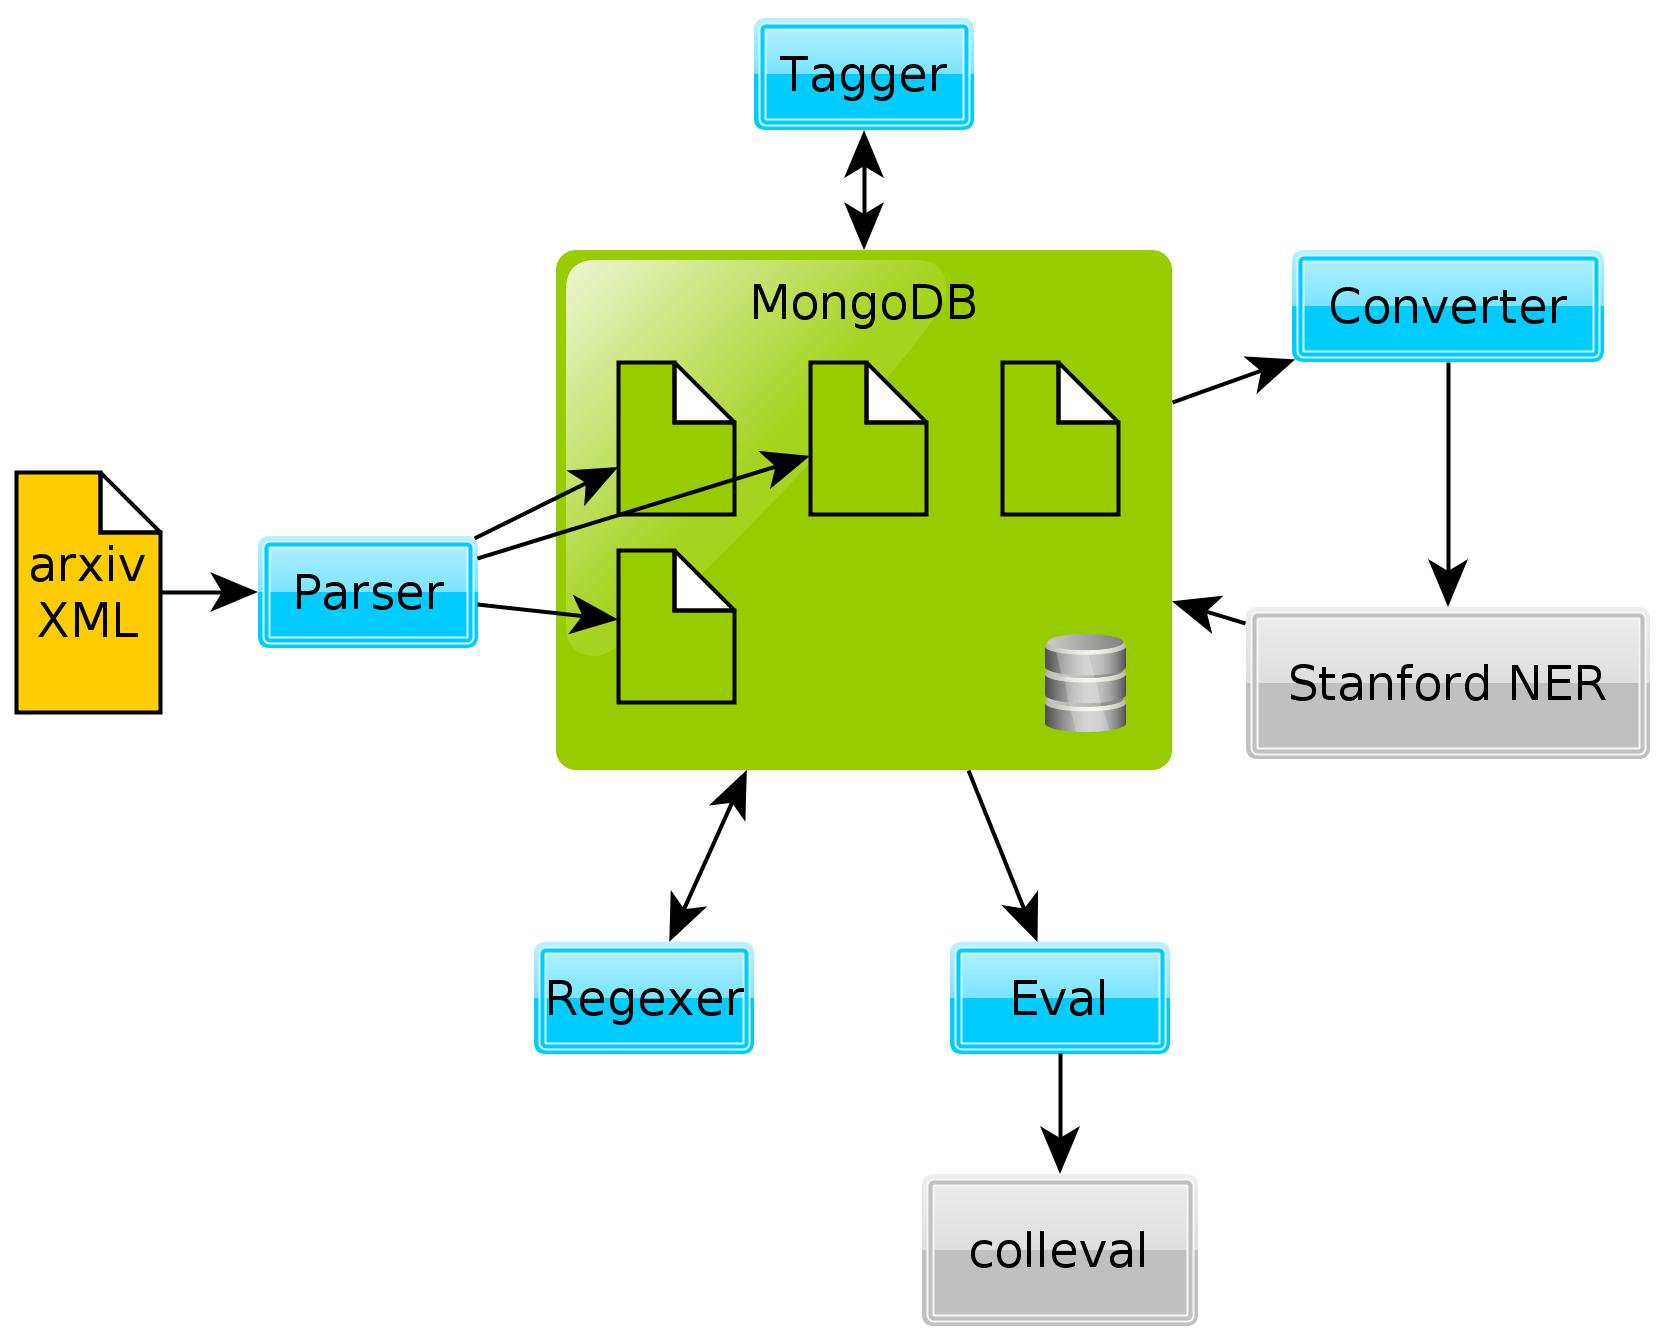
\includegraphics[width=0.7\textwidth]{image/arch.jpg}
  	\caption{Architektur der Evaluationsumgebung\label{arch}}
  \end{center}
\end{figure}

\subsection{Evaluationsmethoden}

\section{Analyse}

\subsection{Ergebnisse der Regelbasierte Erkennung}

\subsubsection*{Nicht erkannte Eigennamen}

\subsubsection*{Falsch erkannte Eigennamen}

\subsection{Ergebnisse der Erkennung mit maschinellem Lernen}

\subsubsection*{Nicht erkannte Eigennamen}

\subsubsection*{Falsch erkannte Eigennamen}

\section{Fazit}

\end{document}

